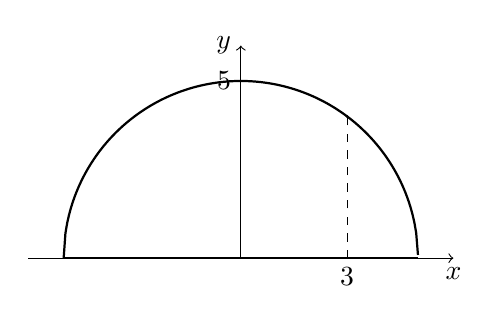
\begin{tikzpicture}[scale=0.45]
    \draw[->] (-6,0) -- (6,0) node[below] {$x$};
    \draw[->] (0,0) -- (0,6) node[left] {$y$};

    \draw[thick, domain=-5:5, samples=200] plot (\x,{sqrt(25-\x*\x)});
    \draw[thick] (-5,0) -- (5,0);

    \draw[dashed] (3,0) -- (3,4);
    \fill (3,4) circle (1.2pt);

    \node[below] at (3,0) {$3$};
    \node[left] at (0,5) {$5$};
\end{tikzpicture}
